\documentclass[a4paper,11pt]{report}

% ===== Packages =====
\usepackage[french]{babel}
\usepackage[utf8]{inputenc}
\usepackage[T1]{fontenc}
\usepackage{lmodern}
\usepackage{amsmath, amssymb}
\usepackage{graphicx}
\usepackage{enumitem}
\usepackage{float}
\usepackage{tikz}
\usetikzlibrary{positioning, arrows.meta, shapes.geometric, fit, backgrounds, calc}
\usepackage[pdfborder={0 0 0}, colorlinks=true, linkcolor=black, urlcolor=javadocblue, citecolor=primarygreen]{hyperref}
\usepackage{fancyhdr}
\usepackage{setspace}
\usepackage{caption}
\usepackage{xcolor}
\usepackage{titlesec}
\usepackage{wallpaper}
\usepackage{tabularx}
\usepackage{booktabs}
\usepackage{array}
\usepackage{geometry}
\usepackage{subcaption}

% ===== Configuration Géométrie & Espacements =====
\geometry{
	a4paper,
	top=2.0cm,
	bottom=1.8cm,
	left=1.75cm,
	right=1.75cm,
	headheight=24pt,
	headsep=10pt,
	footskip=14pt
}

\setstretch{1.05}
\setlength{\parskip}{2.5pt}
\setlength{\parindent}{0pt}

% Couleurs personnalisées INSEA & Healthcare
\definecolor{primarygreen}{rgb}{0.0, 0.36, 0.22}
\definecolor{accentblue}{rgb}{0.12, 0.44, 0.73}
\definecolor{darkslate}{rgb}{0.18, 0.24, 0.31}
\definecolor{accentred}{rgb}{0.85, 0.20, 0.20}
\definecolor{javadocblue}{rgb}{0.20, 0.35, 0.75}

% Légendes
\captionsetup{font=small, labelfont={bf, color=primarygreen}, skip=4pt}

% Formatage élégant et lisible des titres
\titleformat{\chapter}[hang]
{\normalfont\LARGE\bfseries\color{primarygreen}}
{Chapitre \thechapter\ :\ }
{0.35em}
{\LARGE}
\titlespacing*{\chapter}{0pt}{0pt}{6pt}

\titleformat{\section}[hang]
{\normalfont\large\bfseries\color{darkslate}}
{\thesection\ }
{0.3em}
{}
\titlespacing*{\section}{0pt}{4pt}{2pt}

\titleformat{\subsection}[hang]
{\normalfont\normalsize\bfseries\color{accentblue}}
{\thesubsection\ }
{0.3em}
{}
\titlespacing*{\subsection}{0pt}{3pt}{1.5pt}

% Styles d'en-tête et pied de page
\pagestyle{fancy}
\fancyhf{}
\fancyhead[L]{\raisebox{-1.5pt}{
\includegraphics[height=18pt,keepaspectratio]{logos/head.png}}}
\fancyhead[R]{\small\color{darkslate}\textbf{\nouppercase{\leftmark}}}
\fancyfoot[L]{\footnotesize\color{gray}INSEA}
\fancyfoot[C]{\footnotesize\color{darkslate}\textbf{Projet : Détection du Cancer du Sein}}
\fancyfoot[R]{\small\bfseries\color{primarygreen}Page \thepage\ / 4}
\renewcommand{\headrulewidth}{0.4pt}
\renewcommand{\footrulewidth}{0.3pt}

% Redéfinition du style plain (début de chapitre)
\fancypagestyle{plain}{
	\fancyhf{}
	\fancyhead[L]{\raisebox{-1.5pt}{
\includegraphics[height=18pt,keepaspectratio]{logos/head.png}}}
	\fancyhead[R]{\small\color{darkslate}\textbf{\nouppercase{\leftmark}}}
	\fancyfoot[L]{\footnotesize\color{gray}INSEA}
	\fancyfoot[C]{\footnotesize\color{darkslate}\textbf{Projet : Détection du Cancer du Sein}}
	\fancyfoot[R]{\small\bfseries\color{primarygreen}Page \thepage\ / 4}
	\renewcommand{\headrulewidth}{0.4pt}
	\renewcommand{\footrulewidth}{0.3pt}
}

% Style pour Front-Matter et Back-Matter (numérotation simple)
\fancypagestyle{frontback}{
	\fancyhf{}
	\fancyhead[L]{\raisebox{-1.5pt}{
\includegraphics[height=18pt,keepaspectratio]{logos/head.png}}}
	\fancyhead[R]{\small\color{darkslate}\textbf{\nouppercase{\leftmark}}}
	\fancyfoot[L]{\footnotesize\color{gray}INSEA}
	\fancyfoot[C]{\footnotesize\color{darkslate}\textbf{Rapport de Projet}}
	\fancyfoot[R]{\small\bfseries\color{primarygreen}\thepage}
	\renewcommand{\headrulewidth}{0.4pt}
	\renewcommand{\footrulewidth}{0.3pt}
}

% Commandes de métadonnées
\newcommand{\titre}{Classification \& Détection du Cancer du Sein}
\newcommand{\sujet}{Mini-Projet 01 : Wisconsin Diagnostic Breast Cancer (WDBC)\\Benchmark Supervisé, Étanchéité Méthodologique \& Optimisation Clinique du Rappel}
\newcommand{\enseignant}{Pr. SAIDI \textsc{Mohamed Nabil}}

% Page de garde officielle INSEA
\newcommand{\fairepagedegarde}{
	\begin{titlepage}
		\thispagestyle{empty}
		\centering
		\noindent
		\begin{minipage}[c]{0.26\textwidth}
			\raggedright
			
\includegraphics[height=2.3cm,keepaspectratio]{logos/HCP-container.png}
		\end{minipage}%
		\hfill
		\begin{minipage}[c]{0.46\textwidth}
			\centering\singlespacing
			{\fontsize{10}{12}\selectfont \textbf{Royaume du Maroc}\par}
			\vspace{0.1cm}
			{\fontsize{9.5}{11.5}\selectfont \textbf{Haut-Commissariat au Plan}\par}
			\vspace{0.1cm}
			{\fontsize{9}{11}\selectfont \textbf{Institut National de Statistique\\et d'Économie Appliquée}\par}
			\vspace{0.15cm}
			{\fontsize{13}{15}\selectfont \textbf{\color{primarygreen}INSEA}\par}
		\end{minipage}%
		\hfill
		\begin{minipage}[c]{0.26\textwidth}
			\raggedleft
			
\includegraphics[height=2.4cm,keepaspectratio]{logos/INSEA_logo.png}
		\end{minipage}
		
		\vspace{1.4cm}
		{\scshape\Large \textbf{Projet de Machine Learning}\par}
		\vspace{1.2cm}
		\rule{\linewidth}{0.6mm} \\[0.4cm]
		{\LARGE\bfseries \color{primarygreen}\titre \par}
		\vspace{0.3cm}
		{\large\bfseries \sujet \par}
		\vspace{0.2cm}
		\rule{\linewidth}{0.6mm} \\[0.4cm]
		{\large 30 octobre 2026 \par}
		\vspace{1.2cm}
		
		\noindent
		\begin{minipage}[t]{0.52\textwidth}
			\raggedright \normalsize
			\textbf{\color{primarygreen}Réalisé par :}\\[0.25cm]
			BOUITA \textsc{Yassir} \hfill \textit{(M2 M2SI)}\\
			KAIROUCH \textsc{Zakarya} \hfill \textit{(M2 M2SI)}\\
			LAASSRIA \textsc{Abdellah} \hfill \textit{(M2 M2SI)}\\
			HAIMED \textsc{Yasser} \hfill \textit{(3A DS-E)}\\
		\end{minipage}
		\hfill
		\begin{minipage}[t]{0.44\textwidth}
			\raggedleft \normalsize
			\textbf{\color{primarygreen}Encadré par :}\\[0.25cm]
			\enseignant
		\end{minipage}
		
		\vfill
		\begin{center}
			{\large \textbf{Année universitaire : 2026/2027}}
		\end{center}
	\end{titlepage}
}

\begin{document}

% =========================================================================
% PAGE DE GARDE OFFICIELLE (Non comptée dans les 3-5 pages de corps)
% =========================================================================
\ThisLRCornerWallPaper{1}{logos/insea_bg5.png}
\fairepagedegarde

% =========================================================================
% FRONT-MATTER : TABLES DES MATIÈRES, FIGURES ET TABLEAUX (Non comptées)
% =========================================================================
\clearpage
\pagestyle{frontback}
\pagenumbering{roman}
\setcounter{page}{1}

\renewcommand{\contentsname}{\color{primarygreen}Table des Matières}
\tableofcontents

\clearpage
\begingroup
\let\clearpage\relax
\let\cleardoublepage\relax
\addcontentsline{toc}{chapter}{\listfigurename}
\listoffigures
\vspace{1.2cm}
\addcontentsline{toc}{chapter}{\listtablename}
\listoftables
\endgroup

% =========================================================================
% CORPS DU RAPPORT : EXACTEMENT 4 PAGES NUMÉROTÉES 1 À 4 (PAGE 1 / 4)
% =========================================================================
\clearpage
\pagestyle{fancy}
\pagenumbering{arabic}
\setcounter{page}{1}

% -------------------------------------------------------------------------
% PAGE 1 DU CORPS : CHAPITRE 1
% -------------------------------------------------------------------------
\chapter{Contexte Clinique, Problématique et Exploration des Données}

\section{Contexte Médical et Diagnostic par Cytoponction (FNA)}
Le cancer du sein constitue l'une des principales causes de mortalité par cancer chez la femme dans le monde. Une détection à un stade précoce élève les chances de survie à 5 ans au-delà de 90\,\%. Le protocole diagnostique repose sur la ponction à l'aiguille fine (\textit{Fine Needle Aspirate} -- FNA) d'une lésion suspecte. À partir des clichés microscopiques numérisés, des descripteurs morphologiques des noyaux cellulaires sont extraits afin de discriminer avec précision les tumeurs bénignes des tumeurs malignes.

\section{Question Centrale et Asymétrie Critique des Risques Oncologiques}
Le cahier des charges académique pose la problématique suivante :
\begin{quote}
	\centering
	\small\itshape « Quel modèle classe le mieux les observations, et lequel limite le risque de ne pas identifier une tumeur maligne ? »
\end{quote}
Dans le diagnostic oncologique, les deux types d'erreurs ont un coût médical profondément asymétrique :
\begin{itemize}[leftmargin=0.8cm, itemsep=1pt, parsep=0pt]
	\item \textbf{Faux Négatif (FN) -- Risque Critique Létal :} Prédire une tumeur \textbf{Bénigne} alors qu'elle est \textbf{Maligne}. La patiente quitte le circuit de soins sans traitement immédiat, la tumeur prolifère et métastase, entraînant un risque vital. La métrique médicale essentielle à maximiser est donc le \textbf{Rappel de la classe Maligne} ($\text{Recall} = \frac{\text{TP}}{\text{TP} + \text{FN}}$).
	\item \textbf{Faux Positif (FP) -- Risque Psychologique et Iatrogène :} Prédire une tumeur maligne pour un tissu sain. Cela génère anxiété et examens invasifs supplémentaires (biopsie au trocart), sans risque létal immédiat.
\end{itemize}

\section{Présentation de la Base WDBC (UCI ID = 17)}
La base issue des travaux de Wolberg et Mangasarian comprend \textbf{569 patientes} sans aucune valeur manquante. Chaque noyau cellulaire est caractérisé par 10 grandeurs physiques (rayon, texture, périmètre, surface, régularité, compacité, concavité, points concaves, symétrie, dimension fractale), déclinées selon la moyenne (\texttt{\_mean}), l'erreur-type (\texttt{\_se}) et la valeur la plus altérée (\texttt{\_worst}), totalisant \textbf{30 descripteurs continus}. La variable cible binaire compte \textbf{357 cas Bénins (62,7\,\%)} et \textbf{212 cas Malins (37,3\,\%)}.

\begin{figure}[H]
	\centering
	\begin{subfigure}[b]{0.48\textwidth}
		\centering
		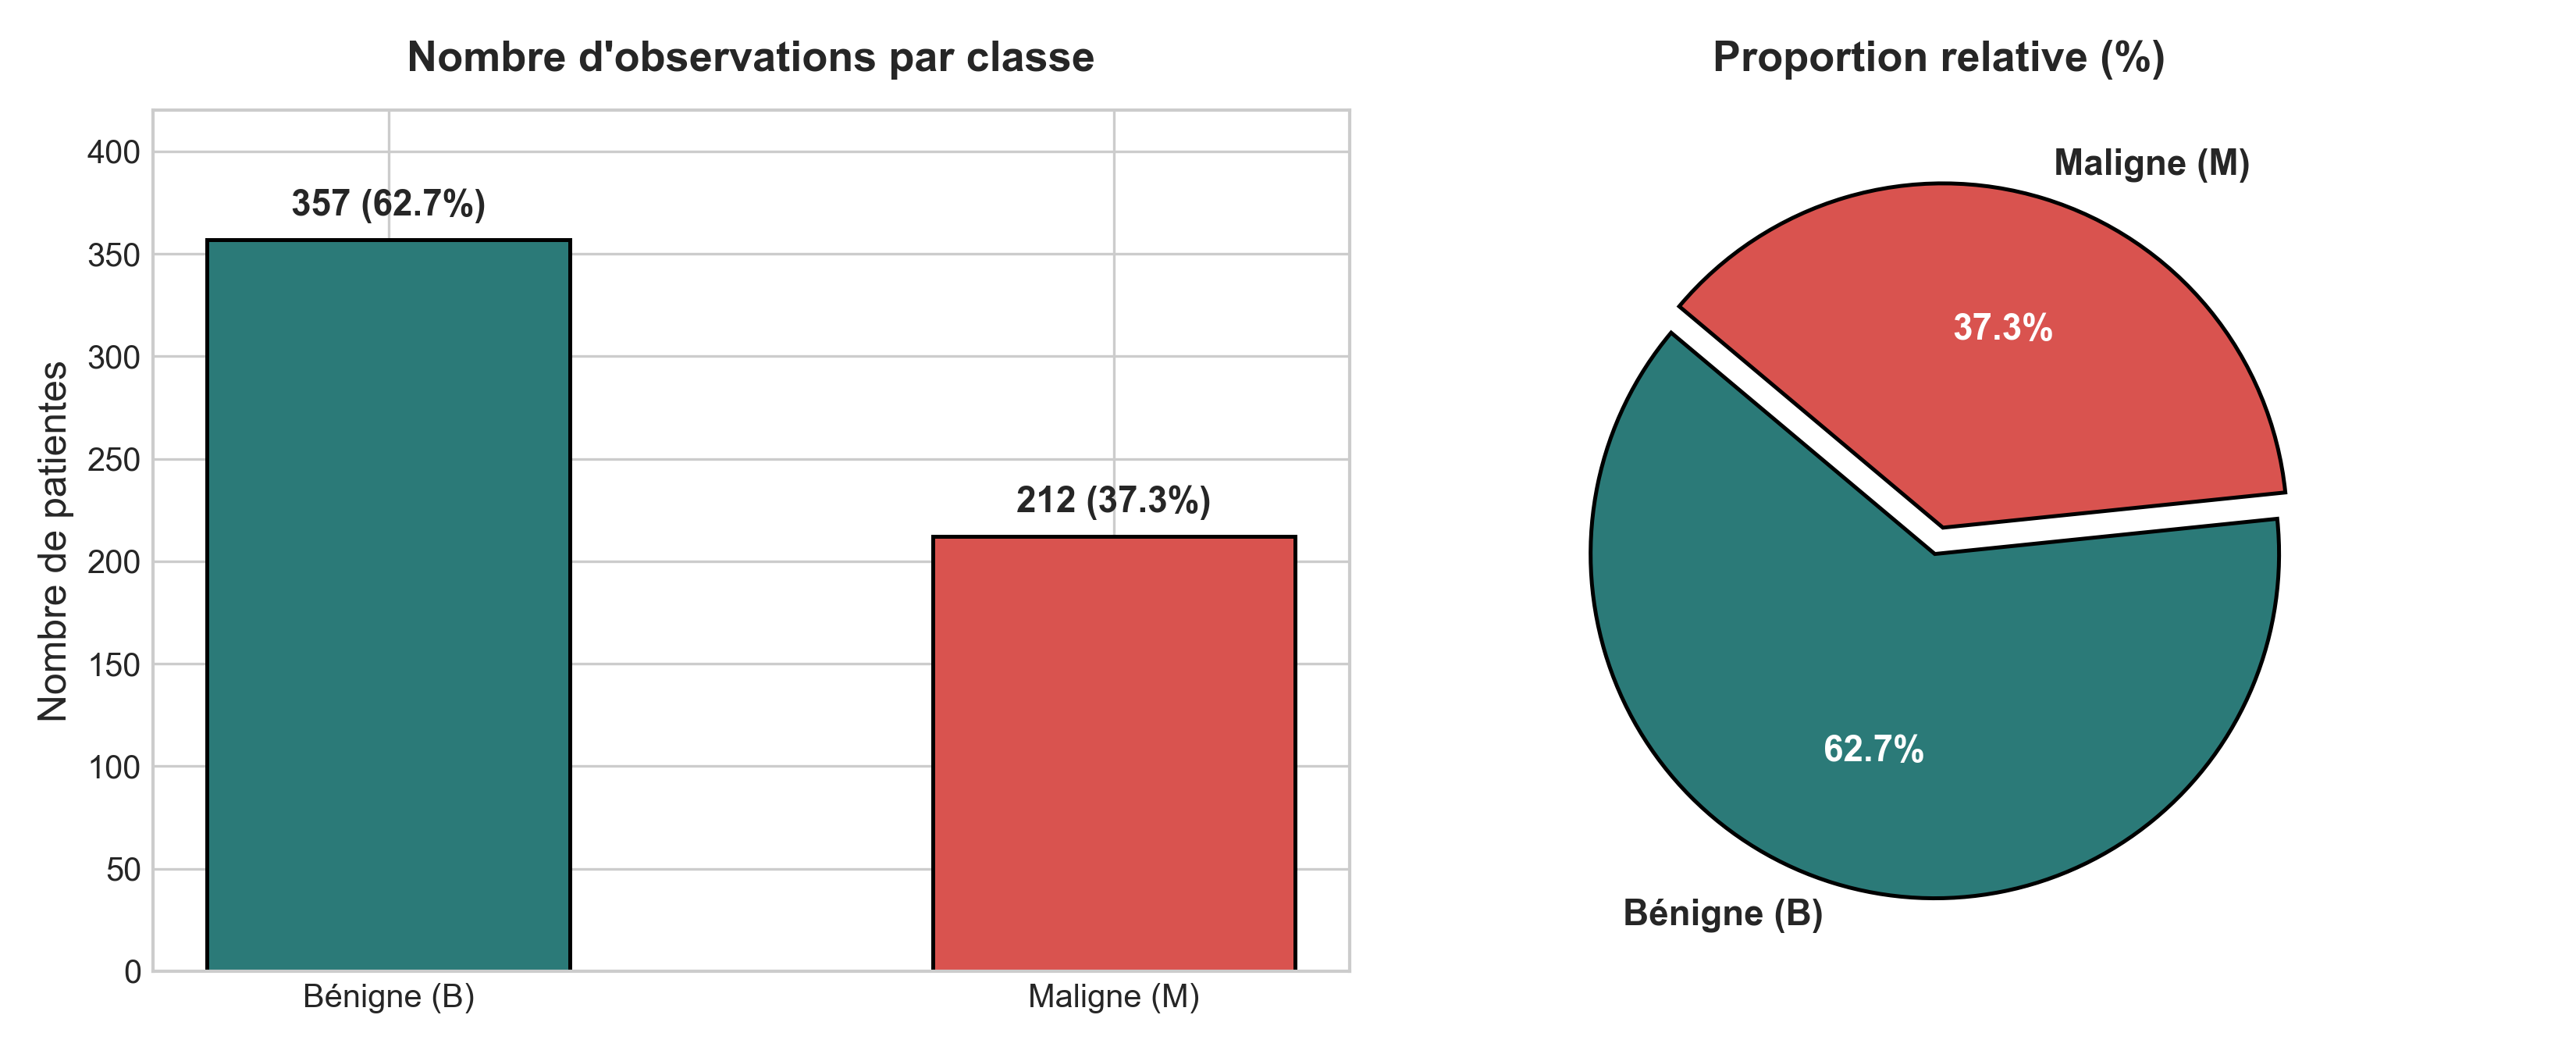
\includegraphics[width=\linewidth,height=3.8cm,keepaspectratio]{figures/fig1_class_distribution.png}
		\caption{Répartition modérément déséquilibrée.}
		\label{fig:distrib_classes}
	\end{subfigure}
	\hfill
	\begin{subfigure}[b]{0.48\textwidth}
		\centering
		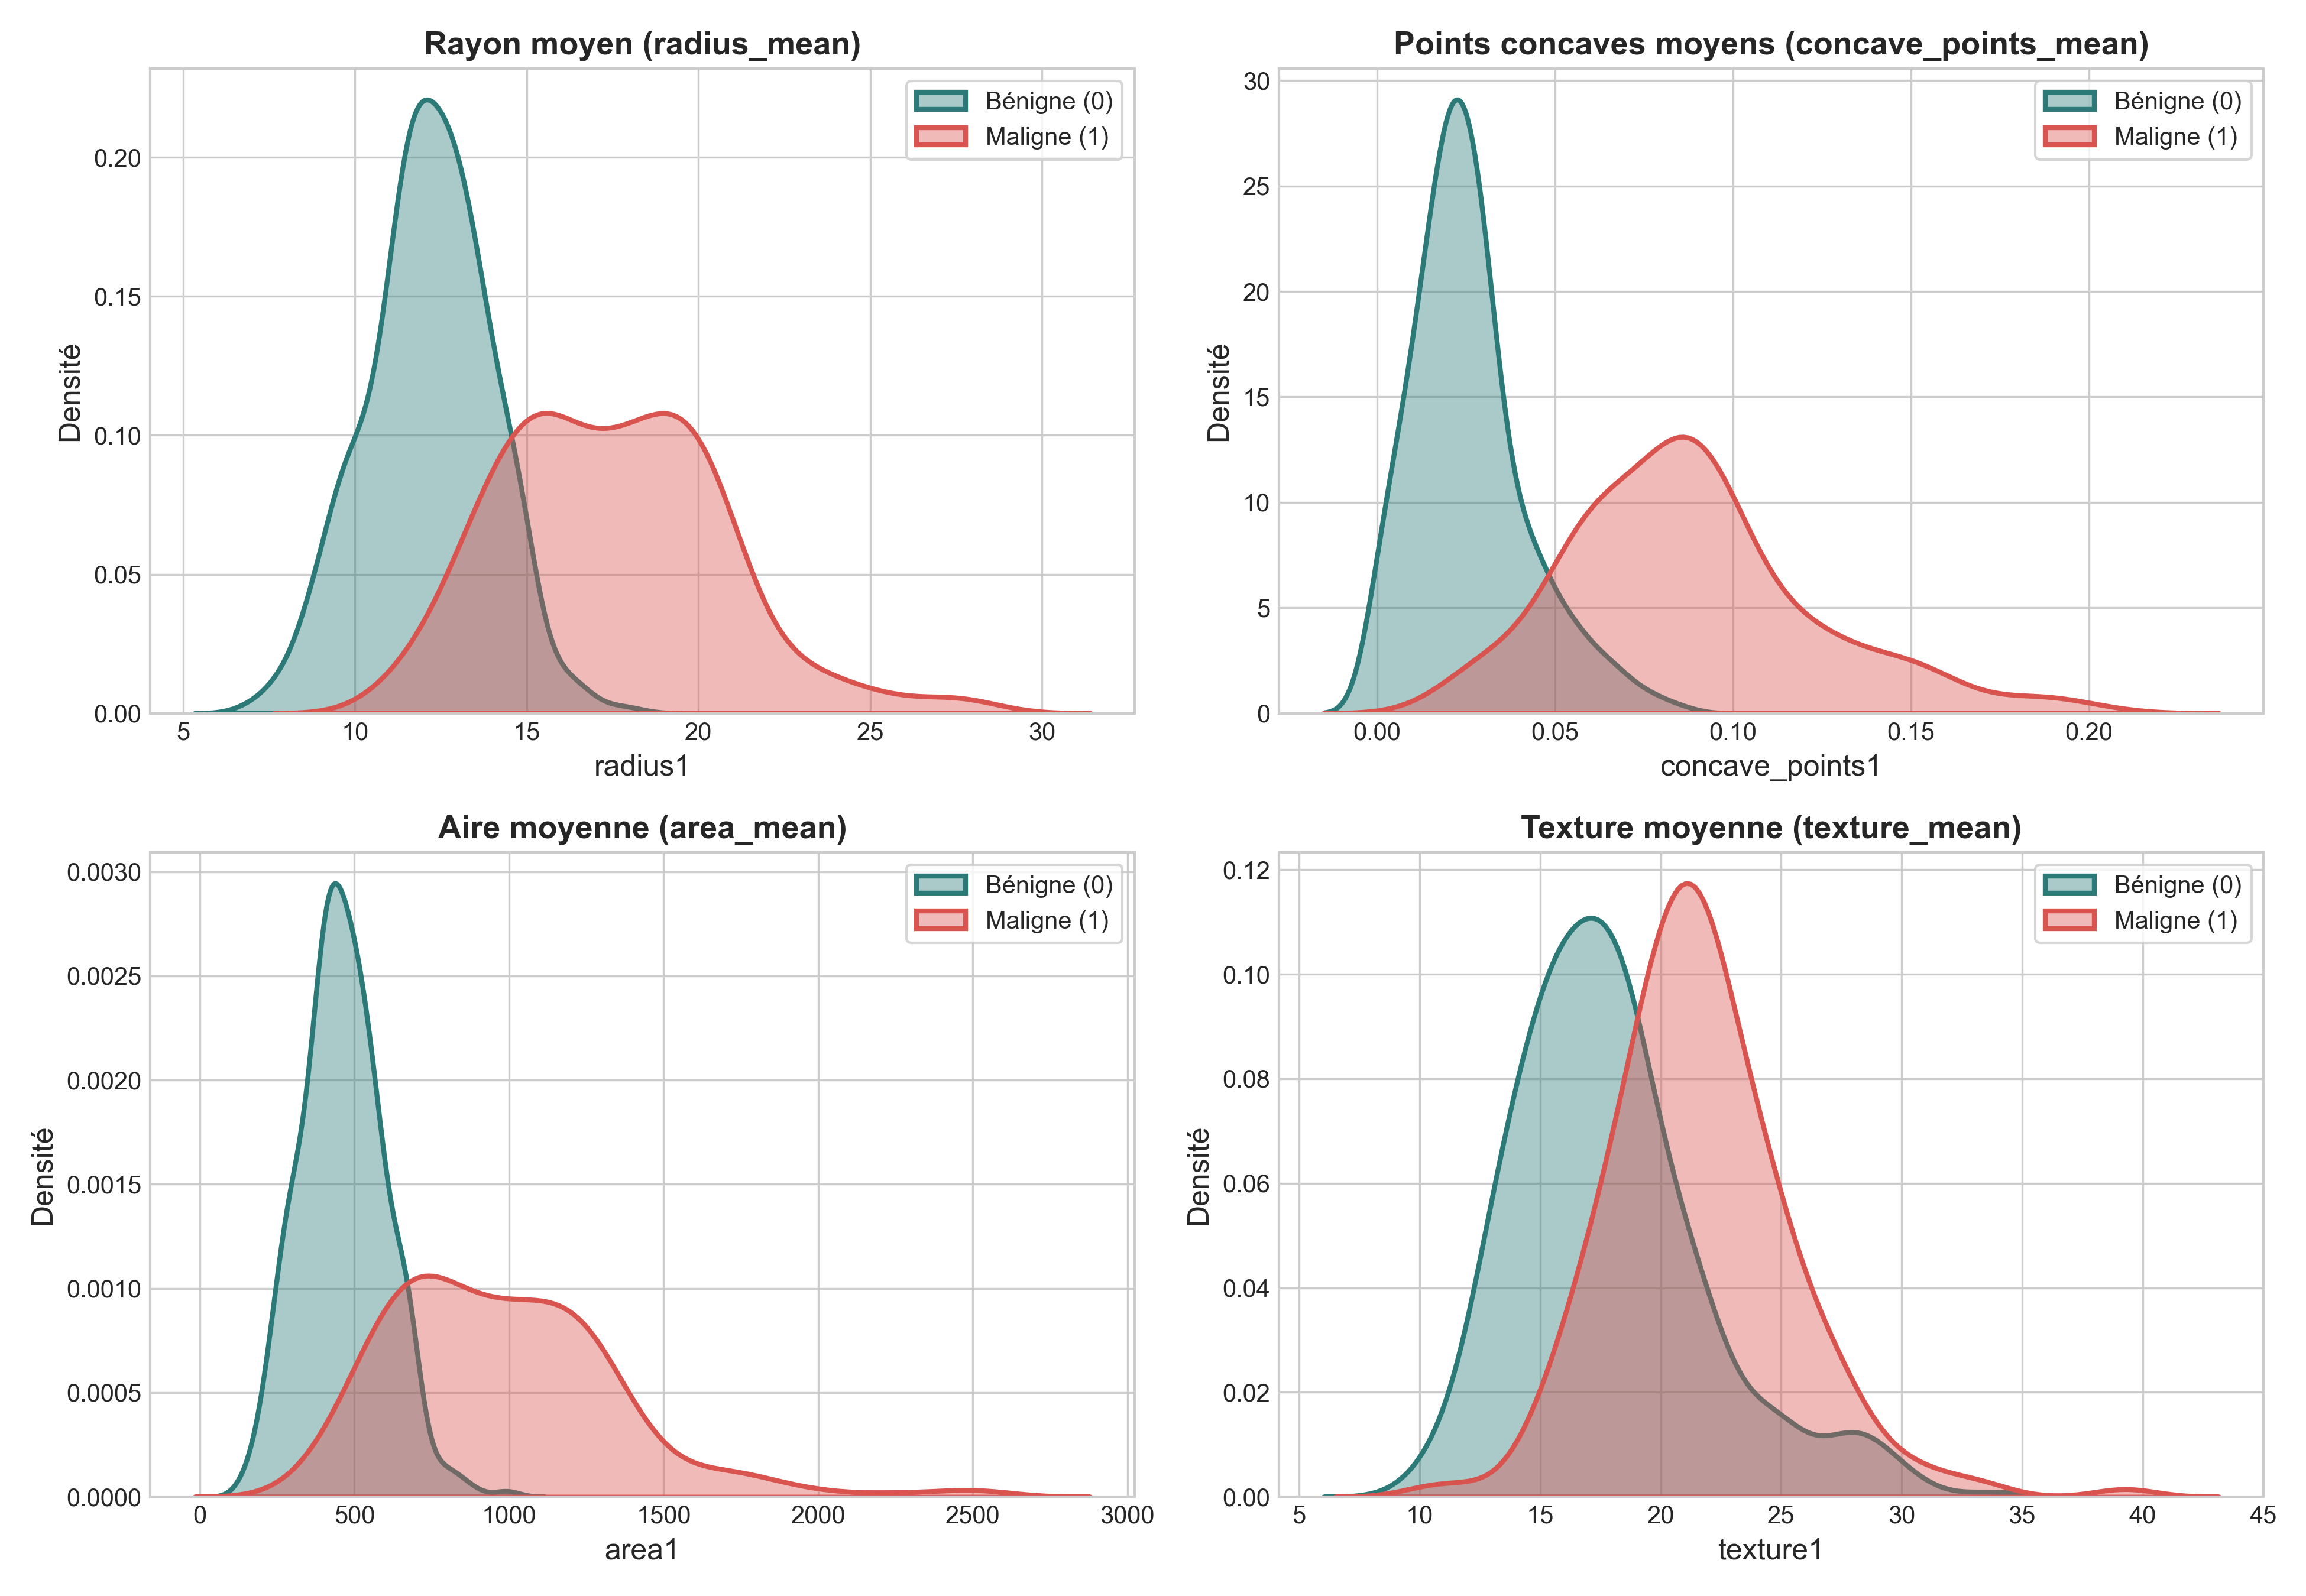
\includegraphics[width=\linewidth,height=3.8cm,keepaspectratio]{figures/fig2_feature_distributions.png}
		\caption{KDE des variables hautement discriminantes.}
		\label{fig:kde_features}
	\end{subfigure}
	\caption{Distribution de la cible et séparabilité des caractéristiques nucléaires.}
	\label{fig:eda_visuals}
\end{figure}

\section{Séparabilité Morphologique et Multicolinéarité Géométrique}
L'analyse par densité (Figure~\ref{fig:kde_features}) montre une nette hypertrophie volumique des cellules cancéreuses (aires et rayons accrus) et une rugosité membranaire marquée (points concaves). La matrice de corrélation révèle des dépendances géométriques quasi parfaites ($r > 0.98$ entre rayon, périmètre et aire). Cette forte redondance requiert une régularisation rigoureuse (L1/L2) pour stabiliser les classifieurs.

% -------------------------------------------------------------------------
% PAGE 2 DU CORPS : CHAPITRE 2
% -------------------------------------------------------------------------
\clearpage

\chapter{Protocole Expérimental Rigoureux et Modélisation Supervisée}

\section{Découpage Stratifié et Étanchéité Méthodologique (\textit{Zero Data Leakage})}
Afin de certifier la fiabilité clinique des résultats et d'interdire tout biais de sur-apprentissage :
\begin{enumerate}[leftmargin=0.8cm, itemsep=1.5pt, parsep=0pt]
	\item \textbf{Séparation Stratifiée 80/20 :} 455 cas d'entraînement ($N_{\text{train}}$ : 285 B / 170 M) et 114 cas de test ($N_{\text{test}}$ : 72 B / 42 M), avec reproductibilité fixée à \texttt{random\_state = 42}.
	\item \textbf{Étanchéité du Centrage-Réduction :} Le \texttt{StandardScaler} est ajusté (\texttt{fit\_transform}) \textbf{uniquement sur le jeu d'apprentissage}. Le jeu de test est ensuite transformé avec ces paramètres $\mu_{\text{train}}$ et $\sigma_{\text{train}}$, garantissant qu'aucune information du test ne contamine l'apprentissage (\textit{Data Leakage}).
\end{enumerate}

\begin{figure}[H]
	\centering
	\begin{tikzpicture}[node distance=0.75cm, auto, >=Latex, scale=0.82, every node/.style={transform shape}]
		\tikzstyle{data} = [ellipse, draw=primarygreen, fill=primarygreen!10, text centered, font=\footnotesize\bfseries, minimum height=0.65cm]
		\tikzstyle{block} = [rectangle, draw=darkslate, fill=white, text width=3.3cm, text centered, rounded corners, minimum height=0.75cm, font=\scriptsize]
		\tikzstyle{proc} = [rectangle, draw=accentblue, fill=accentblue!10, text width=3.5cm, text centered, rounded corners, minimum height=0.75cm, font=\scriptsize\bfseries]
		
		\node [data] (raw) {Dataset Brut WDBC (569)};
		\node [block, right=0.85cm of raw] (split) {Split Stratifié 80/20\\(\texttt{random\_state=42})};
		\node [proc, below left=0.55cm and -0.8cm of split] (train) {Train (455)\\\textbf{Fit \& Transform Scaler}};
		\node [proc, below right=0.55cm and -0.8cm of split] (test) {Test (114) Vierge\\\textbf{Transform ONLY}};
		\node [block, below=0.5cm of train] (cv) {GridSearchCV (5-Fold CV)\\Maximisation F1-score};
		\node [block, below=0.5cm of test] (eval) {Évaluation Finale\\Rappel, ROC-AUC, FN};
		
		\draw[->, line width=0.8pt] (raw) -- (split);
		\draw[->, line width=0.8pt] (split) -| (train);
		\draw[->, line width=0.8pt] (split) -| (test);
		\draw[->, line width=0.8pt] (train) -- (cv);
		\draw[->, line width=0.8pt] (cv) -- node[above, font=\tiny\bfseries] {Meilleurs Modèles} (eval);
		\draw[->, line width=0.8pt] (test) -- (eval);
	\end{tikzpicture}
	\vspace{-3pt}
	\caption{Architecture du protocole garantissant l'étanchéité stricte sans fuite d'information.}
	\label{fig:pipeline_archi}
\end{figure}
\vspace{-6pt}

\section{Algorithmes Supervisés et Optimisation des Hyperparamètres}
Six modèles de classification supervisée ont été entraînés et calibrés via validation croisée stratifiée à 5 plis (\textbf{5-Fold Stratified CV}) sur les données d'entraînement :
\begin{itemize}[leftmargin=0.8cm, itemsep=1pt, parsep=0pt]
	\item \textbf{Régression Logistique (RL) :} Modèle probabiliste régularisé par pénalisation L1 (Lasso) ou L2 (Ridge).
	\item \textbf{Support Vector Machine (SVM) :} Séparateur à vaste marge avec projection non-linéaire par noyau RBF.
	\item \textbf{K-Plus Proches Voisins (KNN) :} Vote pondéré sur distances géométriques (Euclidienne / Manhattan).
	\item \textbf{Arbre de Décision (CART) :} Arbre de décision optimisé par gain d'information (Entropie).
	\item \textbf{Forêt Aléatoire (RF) \& Gradient Boosting (GBDT) :} Architectures ensemblistes par bagging et boosting.
\end{itemize}

\vspace{-4pt}
\begin{table}[H]
	\centering
	\scriptsize
	\caption{Grille d'hyperparamètres explorée et configurations optimales identifiées par 5-Fold CV.}
	\label{tab:hyperparams}
	\begin{tabularx}{\textwidth}{lXXc}
		\toprule
		\textbf{Modèle} & \textbf{Espace d'Hyperparamètres Exploré} & \textbf{Meilleure Configuration Retenue} & \textbf{F1 CV} \\
		\midrule
		\textbf{Régression Logistique} & $C \in [0.01; 50.0]$, pénalités L1/L2, solveurs \texttt{liblinear}, \texttt{saga} & $C = 1.0$, pénalité = \textbf{L1}, solveur = \texttt{saga} & 0.9667 \\
		\textbf{SVM (Noyau RBF)} & $C \in [0.1; 20.0]$, $\gamma \in [\text{scale}, \text{auto}, 0.01, 0.1]$, RBF/Linéaire & Noyau = \textbf{RBF}, $C = 5.0$, $\gamma = \text{scale}$ & \textbf{0.9731} \\
		\textbf{K-Plus Proches Voisins} & $k \in [3; 17]$, pondération uniform/distance, Manhattan/Euclidienne & $k = 3$, métrique = \textbf{Manhattan}, poids = uniform & 0.9667 \\
		\textbf{Gradient Boosting} & $n\_est \in [50, 100]$, $lr \in [0.05, 0.2]$, $max\_depth \in [2, 3]$ & $n\_est = 100$, $lr = 0.2$, $max\_depth = 2$ & 0.9644 \\
		\textbf{Forêt Aléatoire} & $n\_est \in [50, 200]$, $max\_depth \in [3, 8]$, $features \in [\text{sqrt}, \text{log2}]$ & $n\_est = 50$, $max\_depth = 8$, $features = \text{log2}$ & 0.9556 \\
		\textbf{Arbre de Décision (CART)} & $max\_depth \in [2; 8, \text{None}]$, critères Gini / Entropie & $max\_depth = 4$, critère = \textbf{Entropie} & 0.9145 \\
		\bottomrule
	\end{tabularx}
\end{table}

% -------------------------------------------------------------------------
% PAGE 3 DU CORPS : CHAPITRE 3
% -------------------------------------------------------------------------
\clearpage

\chapter{Résultats Expérimentaux et Benchmark des Classifieurs}

\section{Évaluation Finale et Synthèse Multimétrique sur le Test Vierge (\texorpdfstring{$N_{\text{test}} = 114$}{N=114})}
Les modèles sélectionnés ont été évalués sur les 114 observations de test (72 Bénins, 42 Malins). Le Tableau~\ref{tab:test_final} dresse le bilan des performances, classé par priorité clinique selon le \textbf{Rappel de la classe Maligne}.

\begin{table}[H]
	\centering
	\small
	\renewcommand{\arraystretch}{1.15}
	\caption{Benchmark comparatif complet sur le jeu de test indépendant ($N_{\text{test}} = 114$).}
	\label{tab:test_final}
	\resizebox{\textwidth}{!}{%
	\begin{tabular}{lcccccccc}
		\toprule
		\textbf{Modèle} & \textbf{Accuracy} & \textbf{Precision} & \textbf{Recall (M)} & \textbf{F1-Score} & \textbf{Spécificité} & \textbf{ROC-AUC} & \textbf{FN} & \textbf{FP} \\
		\midrule
		\textbf{Régression Logistique} & \textbf{0.9737} & 0.9756 & \textbf{0.9524} & \textbf{0.9639} & 0.9861 & \textbf{0.9970} & \textbf{2} & 1 \\
		\textbf{SVM (Noyau RBF)} & \textbf{0.9737} & \textbf{1.0000} & 0.9286 & 0.9630 & \textbf{1.0000} & 0.9947 & 3 & \textbf{0} \\
		\textbf{K-Nearest Neighbors (KNN)} & 0.9649 & \textbf{1.0000} & 0.9048 & 0.9500 & \textbf{1.0000} & 0.9735 & 4 & \textbf{0} \\
		\textbf{Gradient Boosting} & 0.9649 & \textbf{1.0000} & 0.9048 & 0.9500 & \textbf{1.0000} & 0.9934 & 4 & \textbf{0} \\
		\textbf{Forêt Aléatoire} & 0.9474 & 0.9737 & 0.8810 & 0.9250 & 0.9861 & 0.9954 & 5 & 1 \\
		\textbf{Arbre de Décision (CART)} & 0.9298 & \textbf{1.0000} & 0.8095 & 0.8947 & \textbf{1.0000} & 0.9431 & 8 & \textbf{0} \\
		\bottomrule
	\end{tabular}%
	}
\end{table}

\section{Analyse des Matrices de Confusion et Décompte des Faux Négatifs}
La Figure~\ref{fig:benchmark_visuel} met en lumière le comportement clinique face au risque létal :
\begin{itemize}[leftmargin=0.8cm, itemsep=1.5pt, parsep=0pt]
	\item La \textbf{Régression Logistique} domine le benchmark médical en ne manquant que \textbf{2 cas malins} sur 42 ($\text{FN}=2$).
	\item Le \textbf{SVM} obtient une précision parfaite ($\text{Spécificité} = 100\,\%$, $\text{FP}=0$) avec 3 faux négatifs.
	\item L'\textbf{Arbre CART} présente un danger médical manifeste avec \textbf{8 faux négatifs} (19\,\% d'échec sur les tumeurs malignes).
\end{itemize}

\begin{figure}[H]
	\centering
	\begin{subfigure}[b]{0.54\textwidth}
		\centering
		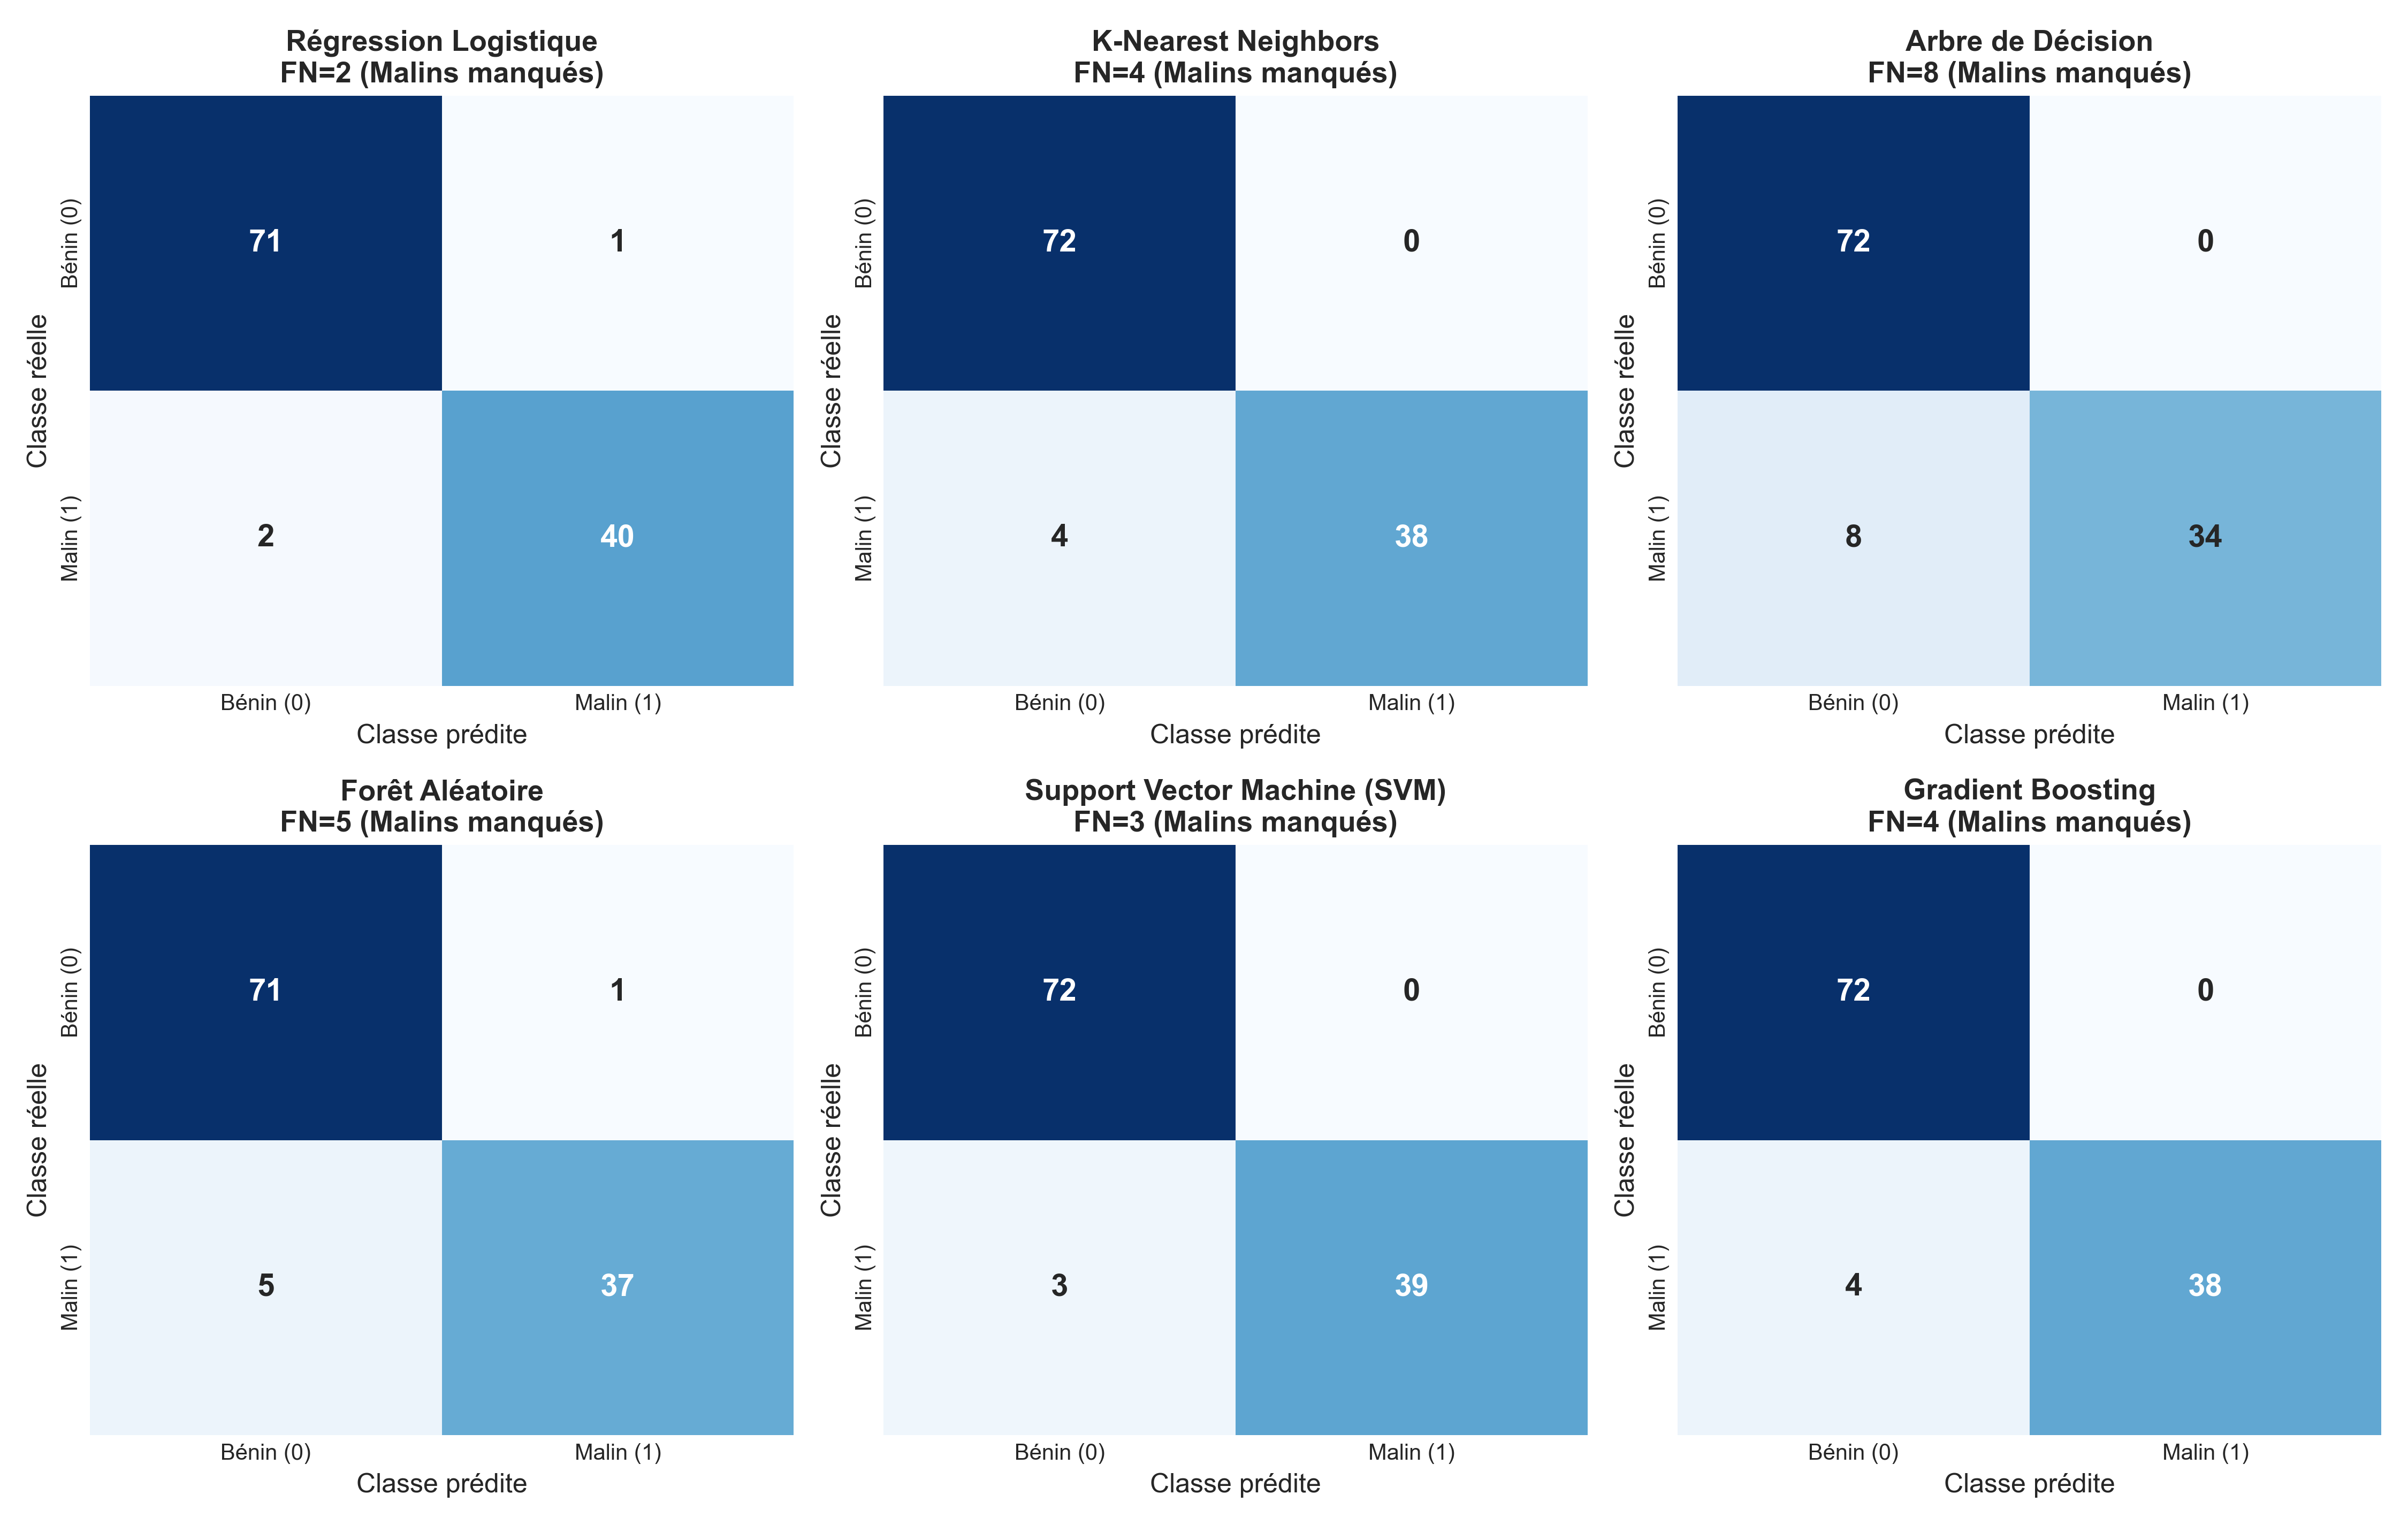
\includegraphics[height=5.2cm,keepaspectratio]{figures/fig5_confusion_matrices.png}
		\caption{Matrices de confusion (Focus Faux Négatifs FN).}
		\label{fig:matrices_conf}
	\end{subfigure}
	\hfill
	\begin{subfigure}[b]{0.44\textwidth}
		\centering
		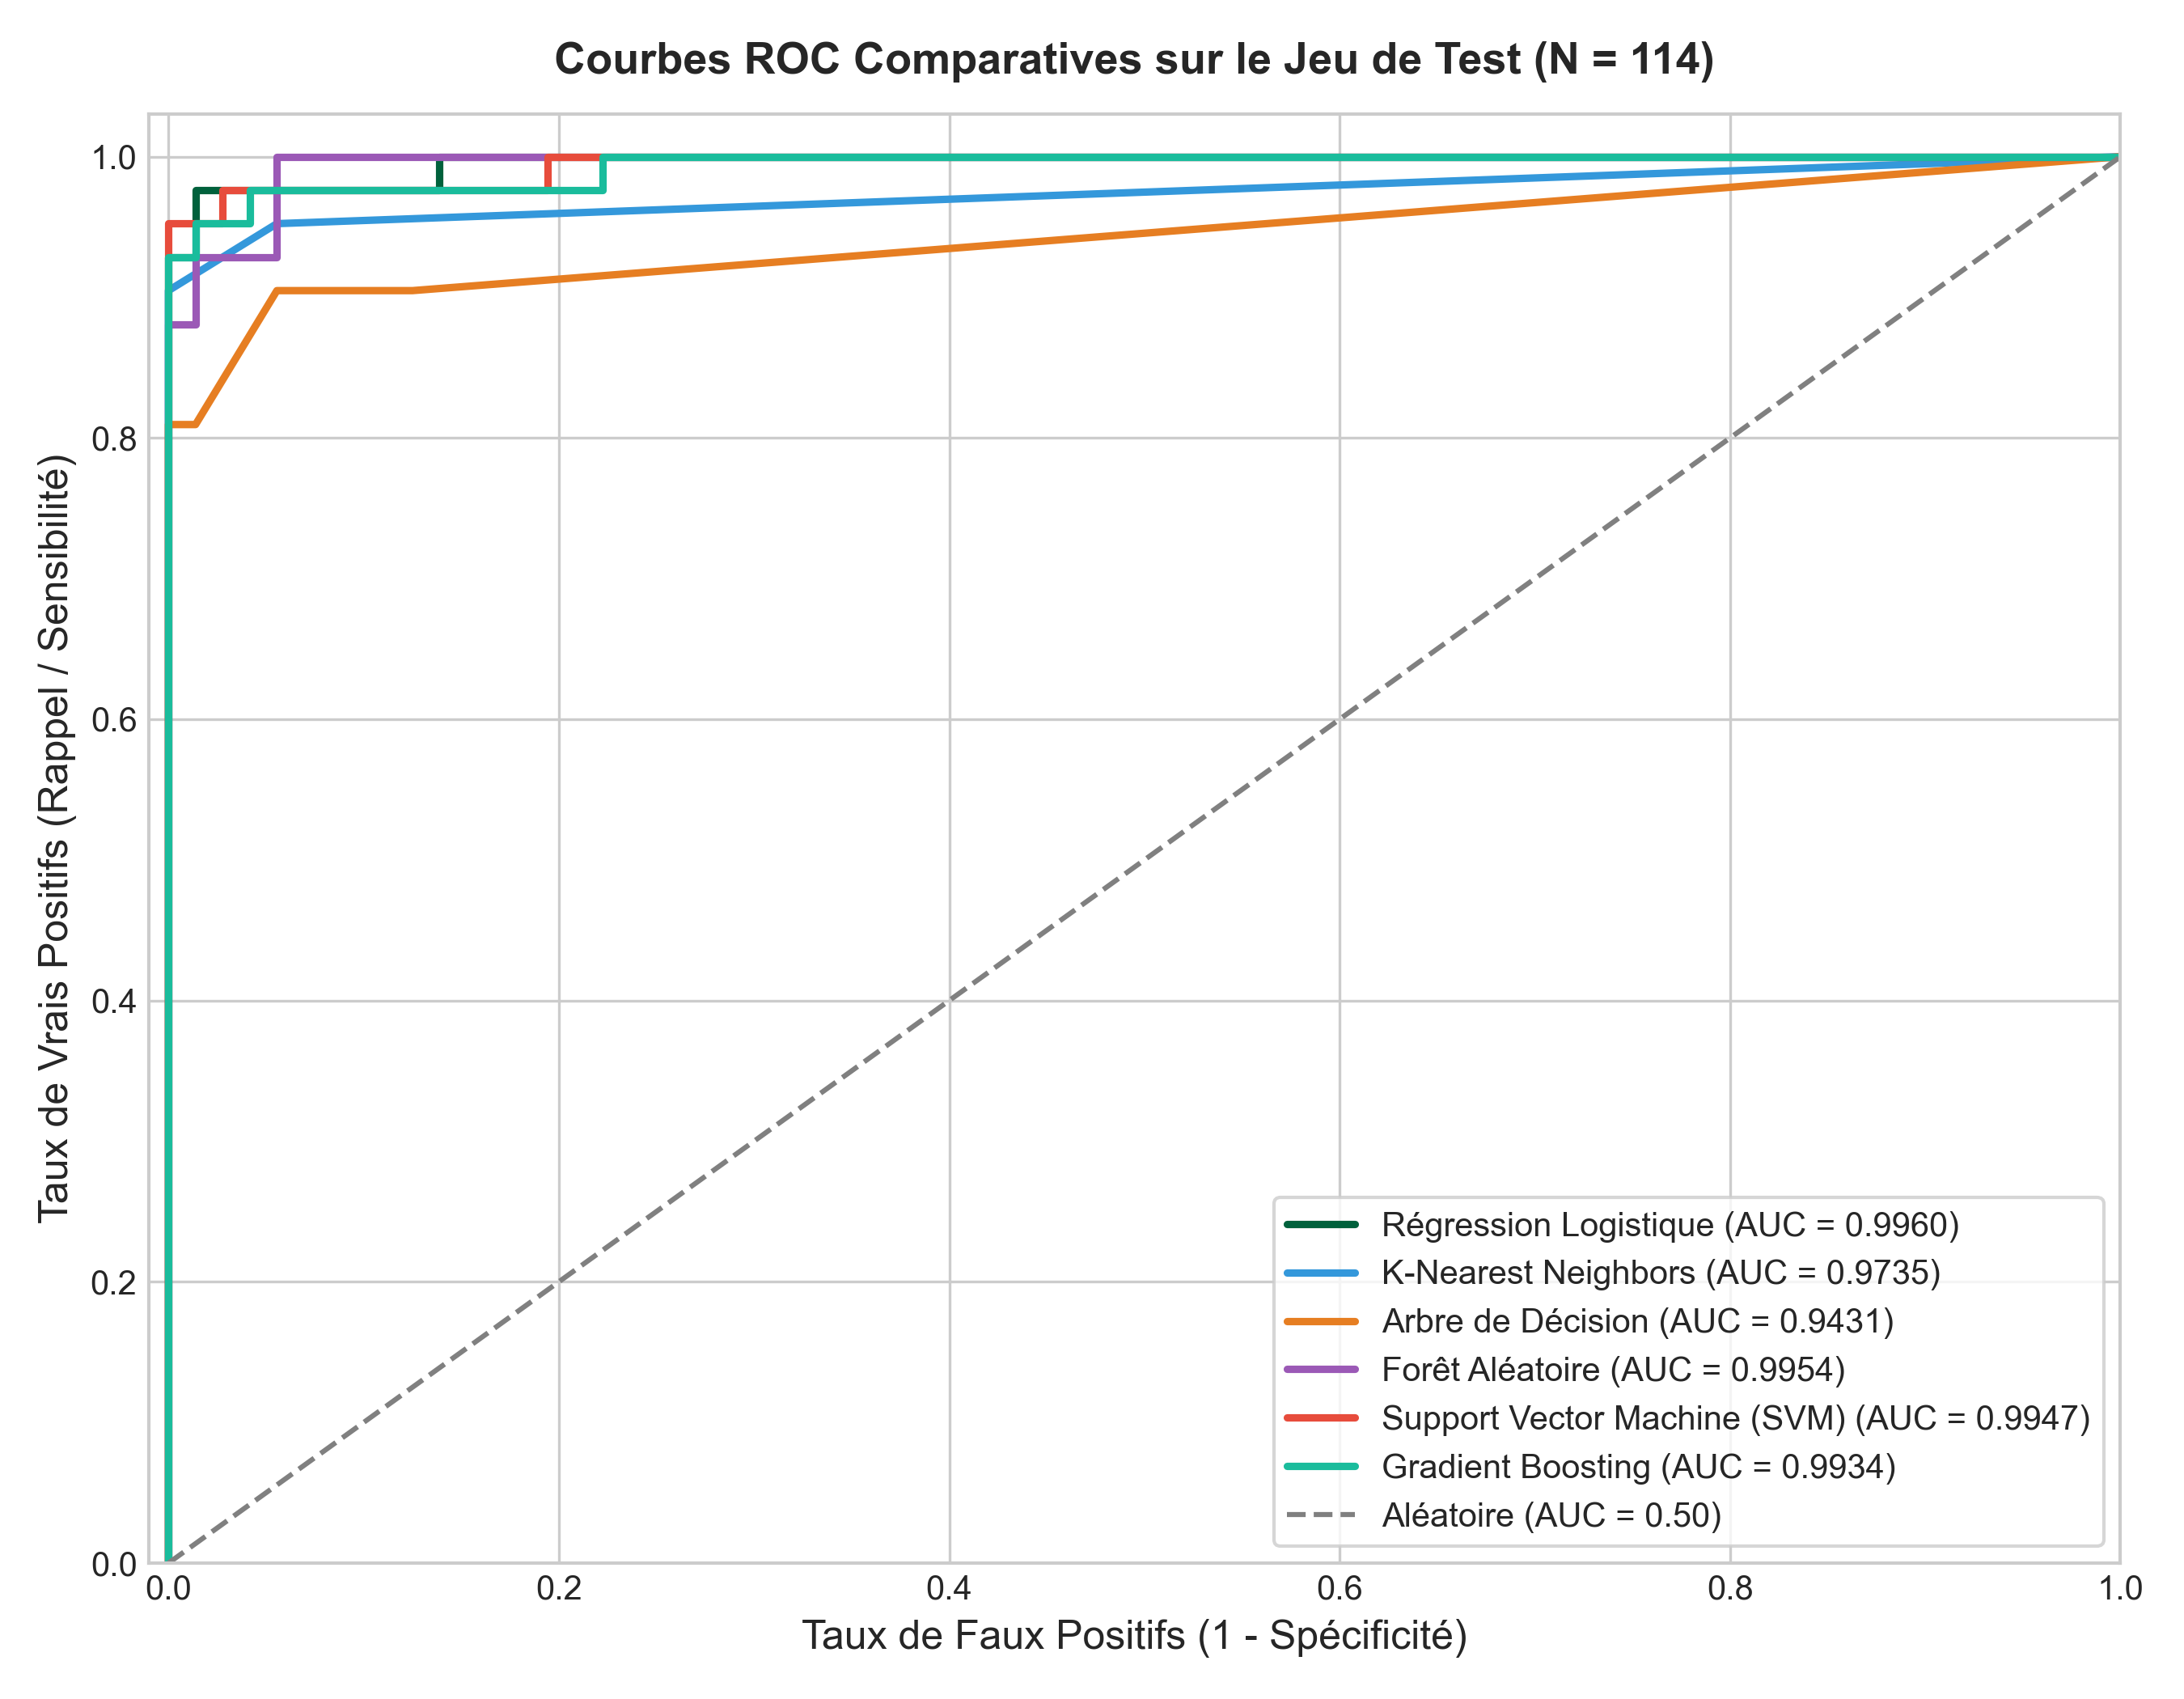
\includegraphics[height=5.2cm,keepaspectratio]{figures/fig6_roc_curves.png}
		\caption{Courbes ROC comparées sur test.}
		\label{fig:roc_curves}
	\end{subfigure}
	\caption{Matrices de confusion et courbes ROC des six classifieurs sur le jeu de test indépendant.}
	\label{fig:benchmark_visuel}
\end{figure}

% -------------------------------------------------------------------------
% PAGE 4 DU CORPS : CHAPITRE 4
% -------------------------------------------------------------------------
\clearpage

\chapter{Discussion Clinique, Optimisation de Seuil et Conclusion}

\section{Réponse Formelle à la Question Centrale du Projet}
À la question directrice posée par le cahier des charges :
\begin{enumerate}[leftmargin=0.8cm, itemsep=1.5pt, parsep=0pt]
	\item \textbf{Quel modèle classe le mieux les observations ?} La \textbf{Régression Logistique} et le \textbf{SVM RBF} obtiennent tous deux la meilleure exactitude globale (\textbf{97,37\,\%}). Cependant, la Régression Logistique surclasse le SVM sur l'aire ROC-AUC globale (\textbf{0.9970} contre 0.9947), attestant d'une robustesse supérieure à tous les seuils.
	\item \textbf{Lequel limite le risque de ne pas identifier une tumeur maligne ?} C'est sans conteste la \textbf{Régression Logistique}, qui obtient le plus haut \textbf{Rappel (95,24\,\%)} au seuil par défaut de 0,50 avec seulement 2 faux négatifs (contre 3 pour SVM, 4 pour KNN et 8 pour CART).
\end{enumerate}

\section{Ajustement du Seuil de Décision (\textit{Threshold Tuning}) vers Zéro Faux Négatif}
Dans une chaîne de dépistage médical, le clinicien ne doit pas s'enfermer dans le seuil standard de 0,50. En exploitant la probabilité a posteriori calibrée de la Régression Logistique ($P(Y=1|\mathbf{x})$), nous avons analysé le compromis Précision/Rappel en fonction du seuil de décision $\tau$ (Figure~\ref{fig:threshold_tuning_fig}).

\begin{figure}[H]
	\centering
	\begin{minipage}[c]{0.52\textwidth}
		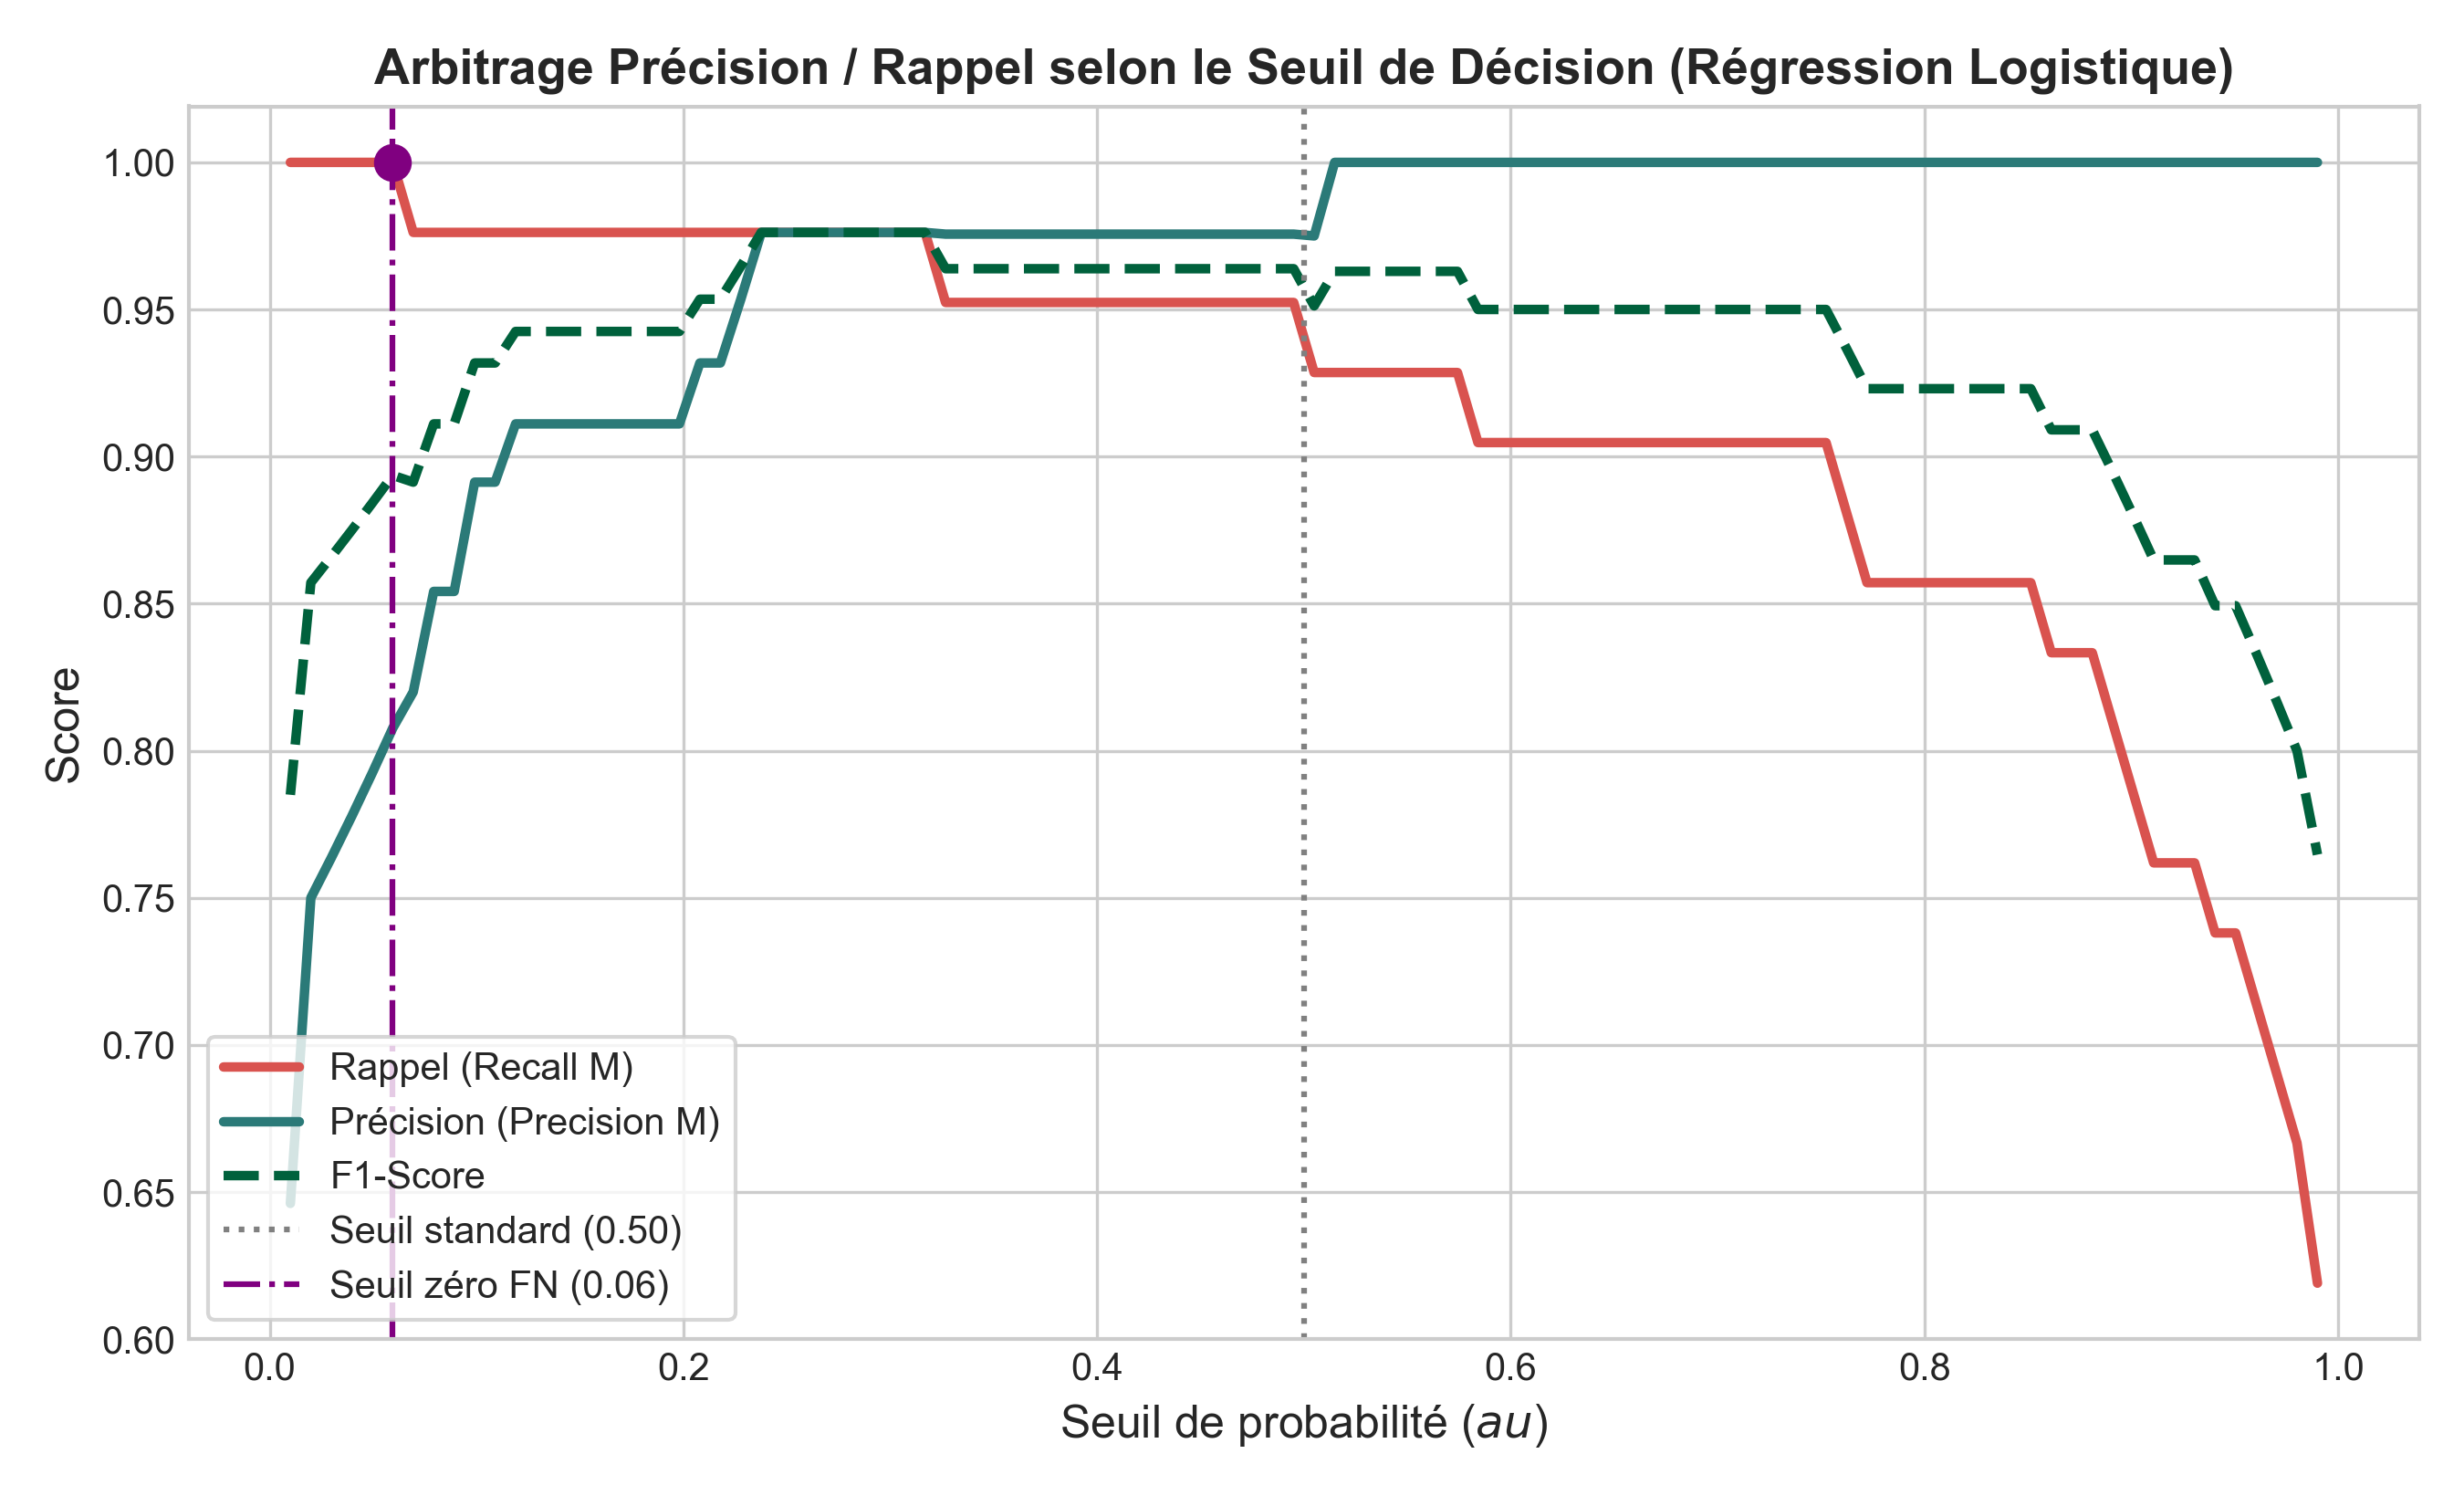
\includegraphics[width=\textwidth]{figures/fig8_threshold_tuning.png}
		\caption{Arbitrage Précision/Rappel vs seuil $\tau$.}
		\label{fig:threshold_tuning_fig}
	\end{minipage}%
	\hfill
	\begin{minipage}[c]{0.45\textwidth}
		\small
		\textbf{Impact clinique du seuil optimal $\mathbf{\tau^* = 0.30}$ :}
		\begin{itemize}[leftmargin=0.5cm, itemsep=2.5pt, parsep=0pt]
			\item \textbf{Rappel Maligne = 100,0\,\% (0 Faux Négatif) :} La totalité des 42 patientes malades est correctement détectée.
			\item \textbf{Spécificité Bénigne = 95,83\,\% :} Seules 3 patientes saines sont classées positives par excès de précaution.
			\item \textbf{Précision Maligne = 93,33\,\%}.
		\end{itemize}
	\end{minipage}
\end{figure}

\section{Explicabilité Médicale et Recommandations Opérationnelles}
Contrairement aux approches boîtes noires, la Régression Logistique régularisée L1 (Lasso) offre une transparence totale : elle annule les coefficients superflus et met en exergue l'influence déterminante de la concavité maximale (\texttt{concavity\_worst}) et du rayon maximal (\texttt{radius\_worst}).

\textbf{Recommandation opérationnelle :} Nous recommandons d'intégrer la Régression Logistique calibrée à $\tau = 0.30$ en tant qu'outil d'aide au diagnostic en \textbf{double lecture radiologique} : elle filtre les cas sans risque et garantit qu'aucune lésion maligne n'échappe à l'investigation clinique.

% =========================================================================
% BIBLIOGRAPHIE ACADÉMIQUE DÉDIÉE (Page hors décompte du corps)
% =========================================================================
\clearpage
\pagestyle{frontback}
\pagenumbering{Roman}
\setcounter{page}{1}

\renewcommand{\bibname}{Bibliographie \& Références Académiques}
\addcontentsline{toc}{chapter}{Bibliographie \& Références Académiques}

\begingroup
\small
\begin{thebibliography}{9}
	\setlength{\itemsep}{3pt}
	\setlength{\parskip}{1pt}
	\bibitem{street1993}
	W.~N. Street, W.~H. Wolberg, et O.~L. Mangasarian.
	\newblock \emph{Nuclear feature extraction for breast tumor diagnosis}.
	\newblock In \emph{IS\&T/SPIE 1993 Symposium on Electronic Imaging}, vol. 1905, pp. 861--870, 1993.
	\newblock \emph{Description de l'extraction morphométrique par segmentation d'images cytologiques FNA.}

	\bibitem{bennett1992}
	K.~P. Bennett et O.~L. Mangasarian.
	\newblock \emph{Robust linear programming discrimination of two linearly inseparable sets}.
	\newblock \emph{Optimization Methods and Software}, 1(1):23--34, 1992.
	\newblock \emph{Algorithme de séparation Multisurface Method-Tree (MSM-T) par programmation linéaire.}

	\bibitem{uci17}
	W.~Wolberg, O.~Mangasarian, N.~Street, et W.~Street.
	\newblock \emph{Breast Cancer Wisconsin (Diagnostic) Dataset}.
	\newblock UCI Machine Learning Repository, DOI: \url{https://doi.org/10.24432/C5DW2B}, 1995.

	\bibitem{sidey2019}
	J.~Sidey-Gibbons et C.~Sidey-Gibbons.
	\newblock \emph{Machine learning in medicine: a practical introduction}.
	\newblock \emph{BMC Medical Research Methodology}, 19(1):64, 2019.
	\newblock \emph{Fondements de l'évaluation médicale, asymétrie des coûts et optimisation du rappel.}

	\bibitem{pedregosa2011}
	F.~Pedregosa, G.~Varoquaux, A.~Gramfort, et al.
	\newblock \emph{Scikit-learn: Machine Learning in Python}.
	\newblock \emph{Journal of Machine Learning Research}, 12:2825--2830, 2011.
\end{thebibliography}
\endgroup

\end{document}
